\newchapter{系统相关技术概述}{System Related Technologies Outline}
  
\newsection{非结构化信息处理}{Unstructed Information Management}

\newsubsection{非结构化信息管理概述}{Introduction of Unstructed Information Management}

在引言中,我们提到过“在当今的社会中,我们周围信息的形态是以非结构化信息为绝对主体的, 也可以说我们接触到的信息中绝大部分是非结构化信息。”,那么什么是非结构化信息?非结构化信息具有什么特点?如何管理非结构化信息?

信息可以分为三类:结构化信息,非结构化信息和半结构化信息。

\begin{enumerate}[topsep=0pt]
  \item [1、] 结构化信息——经过严格标引后的数据,一般以二维表的形式存在。如数据库中的表、各种票据信息等等。\\ 结构化信息又分为以下三种:
  \begin{enumerate}[topsep=0pt]
    \item [(1)] 一维结构化信息。\\ 一维结构化信息可以进一步分为以下两类:
    \begin{enumerate}[topsep=0pt]
      \item [(a)] 第一类一维结构化信息。
      \item [(b)] 第二类一维结构化信息。
    \end{enumerate}
    \item [(2)]二维结构化信息。
    \item [(3)]三维结构化信息。
  \end{enumerate}
  \item [2、] 非结构化信息——没有经过人为处理的不规整的信息。这些信息更加符合人类交流的方式。如新闻报道、科技文献、散文等等。
  \item [3、] 半结构化信息——介于结构化信息和非结构化信息之间的。有一定格式约束,这不同于非结构化信息,但局部上,又按人类自然语法组织信息,与结构化信息又有所区别,例如电报报文,通知、公告、指数统计表等等。
\end{enumerate}

非结构化信息具有如下特点:第一,其格式非常多样;第二,标准是多样性的,不像我们结构化的数据一目了然;第三,在技术上非结构化信息比结构化信息更难标准化和理解。所以存储、检索、发布以及利用需要更加智能化的计算机技术。

基于非结构化信息的特点,将非结构化信息结构化,转化为结构化信息进行管理是一个可行的管理方案,而构建的面向用户的企业非结构化信息管理系统必须具备以下特征:

\begin{enumerate}[topsep=0pt]
  \item [1、] 必须对非结构化信息资源的获取、转换、分析、管理、应用全过程进行分析,提供基于标准工作过程的支持环境。
  \item [2、] 必须提供标准的对外接口、信息描述方法和定制规范降低定制分析机组件和信息应用组件的复杂性。
  \item [3、] 必须提供灵活的信息描述资源模式简化信息结构化信息资源库的构建。
  \item [4、] 采用自然资源技术以支持高质量的“拉式”信息服务和知识抽取。
  \item [5、] 提供对外的标准的接口以支持非结构化信息资源管理系统与企业其他应用系统的集成。
  \item [6、] 提供界面友好的工具方便用户系统管理和应用。
  \item [7、] 其本身应具有易于扩充、动态发展的能力。
\end{enumerate}

图 2-1 为基于UIMA(Unstructured Information Management Architecture)的非结构化信息管理的架构图,具有一定的指导意义:

\begin{newfigure}
  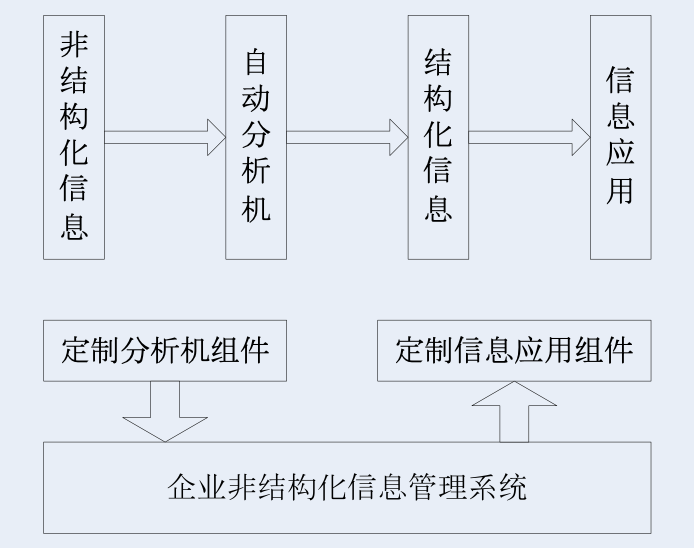
\includegraphics[width=0.3\paperwidth]{figures/figure1.png}
  \caption{企业非结构化信息管理系统应用模式\cite{xdxie-1998}}
\end{newfigure}

在把列名映射到Dundas里面的图例,而行名则映射为Dundas里的轴标签。完成了数据表的映射以后,剩下的就是图表自身形态的改变了。为了实现Dundas形态的改变,我们对Dundas的属性进行了分类和总结,如表2-1所示:

\begin{newtable}
  \caption{Dundas的部分属性表}
  \begin{tabular}{ll}
    \toprule
    属性 & 描述 \\
    \midrule
    图表类型(Chart Type) &	条柱型图表(Bar and Column Charts):条形图、柱状图;\\[2ex]
    线型图表(Line Charts) & 折线图、曲线图、阶梯图;\\[2ex]
    点图表(Point Charts) & 点图、泡泡图;\\[2ex]
    饼图(Pie Charts) & 饼图、圈图;\\[2ex]
    分区图(Area Charts) & 折线分区图、曲线分区图;\\[2ex]
    条柱宽度 (Point Width) &	针对条柱型图表,条柱的宽度。取值从(0,1)。\\[2ex]
    条柱风格 &	针对条柱型图表,有默认、砖型、圆形、棱型、明暗变化\\[2ex]
    数值标签 (Value Label)	& 是否显示数值标签。\\[2ex]
    3D显示	& 是否3D显示。\\[2ex]
    簇状显示 &	是否簇状显示。\\[2ex]
    图例 (Legend) &	字体属性;字号属性;显示位置:图表的左边、右边、上面、下面。\\[2ex]
    标签(Axis) &	字体属性;字号属性。\\[2ex]
    标题(Title) &	字体属性;字号属性。\\[2ex]
    \bottomrule
  \end{tabular}
\end{newtable}

选择算子决定了哪些染色体进入下一代。本算法中采用“轮盘赌”的选择方式,它按照染色体的适应值大小来确定该染色体的被选择概率。如果染色体的适应值越大,其被选中的概率越大。个体 $r_i$ 被选中的概率 $p(r_i)$ 定义如下:

\begin{align}
p(r_i) = Fitness(c_i) / \sum_{j=1}^{pSize} Fitness (c_j), (pSize \mbox{为种群大小}) \tag{公式 2-1}
\end{align}

确定了每个染色体的被选择概率后,系统生成一个在 $[0,1]$ 区间的随机数组,然后与对应染色体的被选择概率比较,如果随机数大于染色体的被选择概率则该染色体被选择,反之被淘汰。

\begin{definition}
如果存在一条从 $V_i$ 到 $V_j$ 的路,称 $V_i$ 是 $V_j$ 的前驱节点,而对于 $(V_i, V_j) \in E$,称 $V_i$ 是 $V_j$ 的立即前驱节点,记为$Vi \in iPred(V_j)$,称 $V_j$ 是 $V_i$ 的立即后继节点,记为 $V_j \in iSucc(Vi)$。
\end{definition}

定义一个公共容器类型的代码如下:

\begin{minted}{c++}
class Container : public Object{
public:
  virtual Object* get();               // 删除并返回当前元素
  virtual void put(Object*);           // 在当前元素之前插入
  virtual Object*& operator[] (size_t);  // 下标
  //…
};
\end{minted}
